\documentclass[12pt,a4paper]{article}
\usepackage{fullpage}
\usepackage{setspace}
    \doublespacing
%\usepackage[usenames,dvipsnames]{xcolor}
\usepackage{hyperref}
\hypersetup{
    colorlinks,
    citecolor=black,
    filecolor=black,
    linkcolor=blue,
    urlcolor=blue
}
\usepackage{dcolumn}
\usepackage{booktabs}
\usepackage{url}
\usepackage{tikz}
\usepackage{todonotes}
\usepackage[T2A]{fontenc}
\usepackage[utf8]{inputenc}
\usepackage[english]{babel}
\usepackage{graphicx}
\usepackage{caption}
\usepackage{subcaption}
\usepackage{afterpage}
\usepackage{xpatch}
\usepackage{csquotes}
\usepackage[style=authoryear, sorting=nyt, dashed=false, maxbibnames=99, backend=bibtex]{biblatex}
\renewbibmacro{in:}{%
  \ifentrytype{article}{}{\printtext{\bibstring{in}\intitlepunct}}}
\renewbibmacro*{volume+number+eid}{
    \printfield{volume}
    \setunit*{\addnbspace}% NEW (optional); there's also \addnbthinspace
    \printfield{number}
    \setunit{\addcomma\space}
    \printfield{eid}}
\DeclareFieldFormat[article]{number}{\mkbibparens{#1}}


\renewcommand*{\bibpagespunct}{\addcolon\space}
\addbibresource{mybib.bib}

\begin{document}



\title{Why are More Trade-Open Countries More Likely to Repress the Media?}
\date{}

\maketitle

Given the conventional wisdom that democratic political institutions drive economic openness \parencite{Milner:2005ci} and vice-versa \parencite{EICHENGREEN:2008gg}, it is surprising that since the 1970s, on average, those countries which have been more open to international trade have had lower levels of media freedom. Although overall economic globalization is positively correlated with media freedom around the world, the bivariate relationship between trade and media freedom is weakly negative. The bottom half of Figure 1 shows that for all available country-years between 1970 and 2011, those which engaged in higher levels of international trade had slightly more repressive media, on average, than those countries which were less open to international trade. This is true in both historically democratic and non-democratic countries, although the difference is most clear among countries with more democratic histories. Given the positive correlation found between media freedom and economic globalization as measured by the KOF index for overall economic globalization \parencite{Dreher:2008dg}, the coincidence of higher trade openness and greater media repression is a surprisingly under-reported empirical puzzle in international and comparative political economy.

\afterpage{
\begin{figure}[t]
    \caption{Media Freedom and Trade vs. General Economic Globalization, 1970-2011}
    \label{absolute}
    \begin{center}
\begin{knitrout}
\definecolor{shadecolor}{rgb}{0.969, 0.969, 0.969}\color{fgcolor}

{\centering 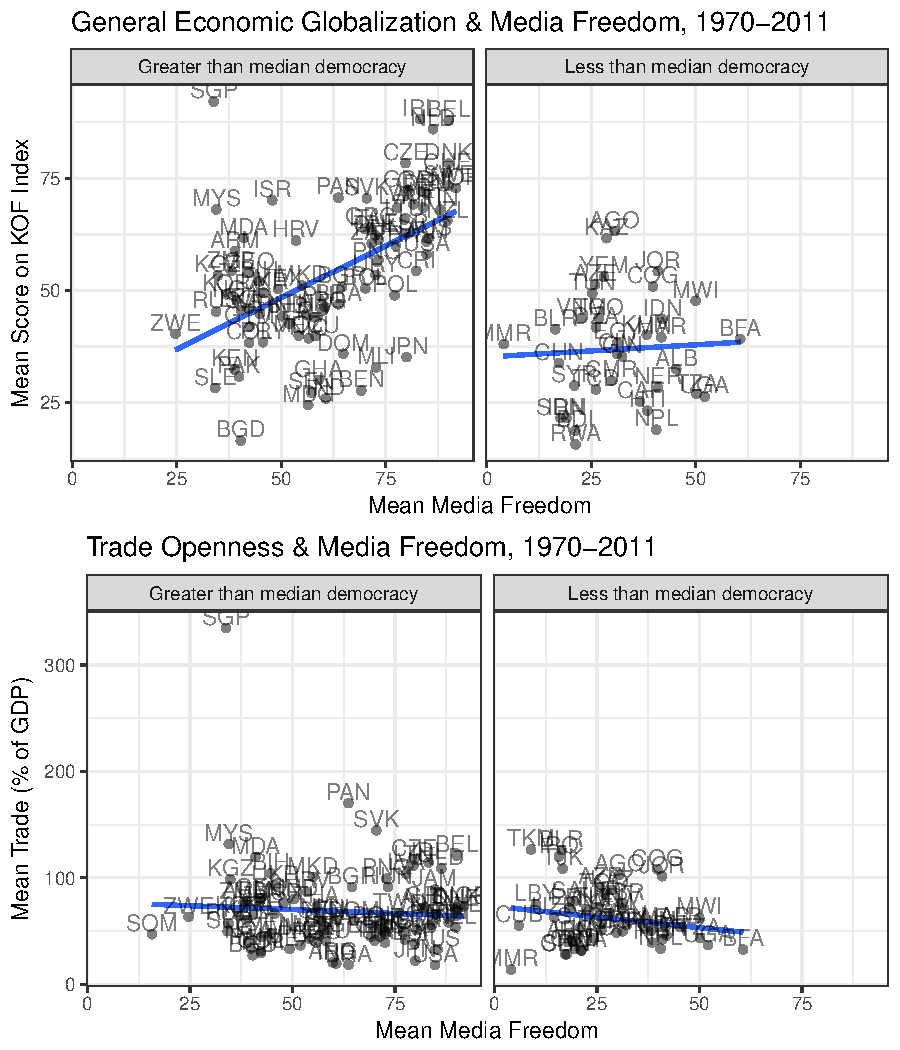
\includegraphics[width=\maxwidth]{figures/Intro-1} 

}



\end{knitrout}
    \end{center}
    \begin{singlespace}
        {\scriptsize{See the section on Data, Method, and Research Strategy for a more detailed description of the data sources. The KOF Index of Globalization (1970-2011) is a 100-point scale reflecting the quantity of international trade and investment policy restrictions as well as flows of trade, FDI, FPI, and income paid to foreign nationals and capital \parencite[43]{Dreher:2008dg}. Media freedom is measured on a dichotomous scale \parencites{Belle:1997wo}{van2000press}. Democracy refers to the 20-point scale from Polity IV \parencite{PolityIVProjectP:2011uq}.
                      }}
    \end{singlespace}
\end{figure}
\clearpage
}

This puzzle points to a larger gap in research on the domestic effects of economic globalization. Scholars of international and comparative political economy (IPE/CPE) have not yet developed a serious theoretical and empirical account of how national media politics are likely to be affected by increasing integration of national economies. Much is known about the effects of economic integration on aspects of domestic politics such as political cleavages \parencites{Rogowski:1987ip}{Rogowski:1989wm}{Hiscox:2002us}{hiscox2002international}, growth rates \parencite{Rodriguez:2001uw}; domestic spending \parencites{Rodrik:1998te}{Burgoon:2001dp}; civil war \parencites{Barbieri:2005uk}{Bussmann:2007vx}, and generic measures of democracy \parencites{EICHENGREEN:2008gg}{Li:2003vj}. But very little is known about how economic integration affects national media politics. One exception is a working paper by Lewis \parencite*{Lewis:qDvYbWlU}, which finds mixed but suggestive evidence that trade openness is negatively related to media freedom and foreign direct investment (FDI) is positively related to media freedom. Other research has considered whether political and civil liberties (broadly including freedom of the media) affect international economic flows \parencite{Adam:2007gn} and the effect of media in economic reform \parencites{Coyne:2004bq}{Islam:2002uc}. Yet scholars of international and comparative political economy have not yet furnished any systematic analysis relating the different components and dynamics of globalization to the domestic politics of media freedom.

This article provides the first systematic investigation of how one key component of economic globalization--international trade--shapes the direction and dynamics of domestic media freedom. On the one hand, economic openness in general might encourage national policymakers to promote media freedom because foreign investors are more likely to invest where information is reliable. On the other hand, because economic liberalization brings distributive conflict which can threaten governments, it also generates incentives for national policymakers to suppress information and communication. A crucial distinction, however, is that while international investors have a stake in the transparency of foreign countries, international traders do not. Therefore, I argue that trade openness should have a negative effect on media freedom because, in contrast to investment, trade brings no pressures which would counter-balance the repressive tendency generated by liberalization.

To test these expectations, I use a mixed-methods research design combining statistical analysis of a large panel of countries from 1972 to 2003 and qualitative process-tracing on the cases of Argentina and Mexico.\footnote{For a full list of countries, see Table 3 in Supplementary Information.} Binary time-sectional, cross-series (BTSCS) analyses provide evidence that, unique among the components of globalization considered here, trade levels have a robustly negative association with media freedom in the long-run. Additionally, qualitative process-tracing on the cases of Argentina and Mexico in the 1990s, selected as relatively hard cases of consolidating democracies which for that reason predict media freedom, each provide some illustration of the mechanism relating trade openness to media repression.

The article makes three main contributions to research on the domestic effects of economic globalization and state-media relations. First, this article provides the first systematic investigation of an important but neglected political-economic relationship, and points to a new set of questions regarding the globalization-media nexus for political economy and media research agendas. Second, the findings contribute to research on the domestic politics of economic globalization and in particular research on the larger globalization-democracy nexus, highlighting a specific causal path through which economic liberalization can call forth media repression as a troublingly anti-democratic technique for negotiating domestic political conflicts. Third, the article will be of interest to scholars of state-media relations and public actors interested in media freedom because very little media research to date has systematically accounted for the ways in which international economic pressures shape states' tendencies toward or away from media freedom.

The article proceeds in five sections. The first section reviews previous research at the intersection of globalization, democracy, and the media. The second section presents a simple informal model of a national policymaker facing domestic backlash for the distributive conflicts brought on by an increase in economic openness, and deducts one main hypothesis regarding the effect of trade openness on media freedom. The third section explains the data, methods, and research strategy. The fourth section presents and discusses the quantitative and qualitative findings, and the fifth section concludes.

\section{Globalization, Democracy, and Media}

Previous research provides strong reasons to expect the global integration of markets to exert pressures on institutions of democracy, but there remains much theoretical uncertainty about the degree to which these effects are positive or negative. Many have argued that economic globalization generates economic growth which strengthens democratic institutions \parencites{Baghwati:1997vy}{Im:1996cl}, increases incentives for peace \parencites{Baghwati:1997vy}{Oneal:1999fc}, or diffuses democracy as a norm (Kant [1795] \cite*{Kant:1983uf}; \cite{Limongi:1996dr}). On the other hand, many have argued that economic globalization is negatively associated with democracy because it rewards efficiency rather than popular sovereignty \parencites{Huntington:1975vt}{Lindblom:1977ue}{Cammack:1998gf}, or because leaders may prefer to repress rather than compensate the domestic losers from increased openness \parencite{Adsera:2002vt}.\footnote{See \cite{Milner:2009hi} for a review of these debates.} Within the general debate surrounding the globalization-democracy nexus, some researchers such as Li and Reveuny \parencite*{Li:2003vj} have sought greater clarity by disaggregating the distinct types of international economic flows and considering them separately, but relying on standard aggregate measures of democracy. Li and Reveuny find that trade and portfolio capital have negative effects on democracy, while FDI and democratic norms have a positive effect, but their dependent variable of democracy is calculated with the common procedure of subtracting the Polity autocracy score from the Polity democracy score. Thus, despite much research on the relationship between economic globalization and democracy, and despite evidence that disaggregation is fruitful for understanding this nexus of relationships, relatively little is known about how different international economic flows affect the various institutions which separately constitute what we know as democracy.

In particular, very little research to date queries whether and how economic globalization shapes state policies regarding domestic media freedom. One exception is Lewis \parencite*{Lewis:qDvYbWlU}, who finds that FDI inflows are positively associated with media freedom, trade levels are negatively associated with media freedom, and portfolio capital inflows have no discernible effect on media freedom. However, Lewis considers only levels of trade and year-by-year inflows of FDI and portfolio capital, whereas recent research shows that the distinction between flows (year-to-year movements) and stocks (the sum of all previous flows) is crucial in researching the effects of foreign investment on repression \parencite{Sorens:2012hc}. As discussed above, Antonis and Fillapaois \parencite*{Adam:2007gn} consider the effect of civil liberties such as media freedom on FDI, but not whether any aspect of economic globalization affects civil liberties.

However, previous research on the relationship between markets and media more generally provides a basis for theorizing the relationship between economic integration and media freedom. Broadly, one tradition argues that the spread of markets and freer media are positively associated \parencites{Habermas:1991vg}{Islam:2002uc}{Islam:2003tu}. However, an opposite tradition suggets that markets and the logic of profits and efficiency create incentives for authoritarianism \parencite{Huntington:1975vt}. With respect to media politics in particular, Gehlbach and Sonin \parencite*{Gehlbach:2011ky} show that larger advertising markets are associated with nationalization of private media because, they argue, the benefits of state control increase with the advertising market. If economic liberalization tends to enlarge advertising markets by spurring economic growth, then liberalization might increase the state's incentives to repress private media just as it increases incentives to nationalize it. Furthermore, international economic integration brings the threat of social and political backlashes \parencite{Bussmann:2007vx}, which may require the state to compensate the domestic losers from globalization \parencite{Rodrik:1998te} or, alternatively, repress them \parencite{Adsera:2002vt}.

On the other hand, the literature on ``competitive authoritarianism'' suggests that increasing economic interdependence is one of the forces which has increasingly rendered traditional authoritarian repression unfeasible \parencite[60, 62]{Levitsky:2002gx}. As a country becomes increasingly integrated with the world economy, it increases the costs of overt authoritarianism by increasing the salience of international opinion, increasing the voice of domestic opposition, and increasing the number of domestic actors affected by international perceptions \parencite{Levitsky:2006ex}. For example, Fujimori in Peru in 1992 and Putin in Russia in 1993 failed in their efforts to overtly circumvent the legislature in part due to such international pressures \parencite[56]{Levitsky:2002gx}. International pressures against overt authoritarianism force regimes to adopt formally democratic institutions such as elections, but often leaves them free to violate human rights and civil liberties. For example, in the US-Mexico negotiations leading up to the North-American Free Trade Agreement, Mexican leaders made significant changes to present a front of democracy and respect for human rights to encourage investors, but there was no specific or formal conditionality which would have prohibited or even discouraged the repression of civil liberties if necessary.

At the same time, Levitsky and Way highlight the media as one of the four main arenas in which incumbent governments can contest and subvert international pressures to democratize. Competitive authoritarian governments may permit a formally independent and relatively free media, as in Peru, Serbia, Panama, or Nicaragua during the late 1980s and much of the 1990s, while engaging in alternative, more subtle tactics of repression, such as manipulative adminstrations of the law or tax code \parencite[53, 58]{Levitsky:2002gx}.

While economic integration engenders distributive conflicts which tempt states to repress certain domestic groups at the same time it disincentivizes certain overt techniques of repression, governments around the world increasingly engage in strategic, authoritarian interventions into domestic media politics. Corrales and Westhoff \parencite*{Corrales:2006vz} find, for instance, that authoritarian regimes are more likely to develop television than internet, because television is more easily controlled. Additionally, many authoritarian regimes welcome the internet but actively pursue techniques of information control and manipulation on the internet in a networked fashion \parencites{MacKinnon:2011id}{Pearce:2012fm}. These findings show that however much economic integration is making certain forms of repression obsolete, newer and more subtle techniques of media repression remain both attractive and viable.

As Antonis and Fillapaois point out, and as Lewis also argues, research on the relationship between globalization and democratic institutions likely shows contradictory results because different international economic flows exert different pressures. In light of this, I restrict my focus to international trade specifically to better understand the puzzling bivariate relationship between trade and media freedom highlighted in the first section. The following section provides a more deductive account of the expected effect of international trade on media freedom.

\section{Theory and Hypotheses}

Based on the review of previous research regarding the domestic political effects of international economic flows and the media politics of competitive authoritarianism, I develop a simple, informal model of how state-media relations should respond to international trade in particular. Consider a state which experiences a variable increase in some inward, international economic flow of trade, FDI, or FPI. This increased flow should increase the income of certain domestic groups and decrease the income of others, according to well-developed open-economy expectations (discussed below). The increased economic flow can be thought of as random and exogenous or the result of conscious state policy such as lowering tariffs. After experiencing the international shock, the media, if free to do so, would be expected to report on its causes and effects and therefore increasing public awareness of its distributive implications. Clearly, to the degree the media are not free to report on the international shock, they would not do so and public awareness of the distributive implications would remain lower than if the media had been free. If they are well-informed, a domestic group which experiences a negative income shock from economic liberalization would demand that the policymaker either close the domestic economy or compensate the group for its income loss, or else face rebellion. This “rebellion” could be electoral if the state is a democracy or a violent insurgency if the state does not have institutions to facilitate peaceful change. If the media is not free to report on the political context and consequences of the international shock, the group which suffers an income loss would be less likely to mobilize around it. In this simple informal model, it is easy to see why free media are essential for domestic losers from globalization to exercise power in the domestic politics around the distributive outcomes of economic globalization. Where there is a free media, domestic losers from globalization are more likely to hold policymakers accountable because they are more likely to be informed and more likely to mobilize around this issue. Where the media are repressed, the losers from globalization should be less able to exact concessions or compensations from policymakers because they will be less informed and therefore less mobilized around this issue.

After increased international exposure occurs, the policymaker would prefer not to compensate the domestic group but prefers compensation to facing rebellion or closing the economy to \emph{ex ante} levels. The policymaker can close the political process to any competitors to obviate the political pressure to compensate them \parencite{Adsera:2002vt}, but the higher their level of integration, the more costly are overt types of repression \parencite{Levitsky:2002gx}. Supposing that a policymaker can choose among compensating the aggrieved domestic group, excluding competitors from the political process, or engaging in some repressive practices which vary on a continuum from overt to covert. In effect, we can conceptualize their utility function as including a penalty on overtness which increases with the country's economic integration, such that there is decreasing utility to overt forms of repression such as outright exclusion from the political process or government killings but this disutility approaches zero for repressive tactics which are relatively obscure such as the selective prosecution or financial targeting of opponents.

Among the less visible ways of exercising anti-democratic control, information-communication control will be uniquely attractive for the policymaker. This is because not only are repressive media tactics less severe than mass killings or canceling elections, but because control of the media could potentially tame international judgments independently by shaping what gets reported internationally. That is, control of the media can first minimize policymaker accountability for the adjustment costs of liberalization by suppressing domestic dissent, but policymakers could also reasonably expect that suppressing information at home would decrease the flow of negative information abroad, promoting their international image in part by repressively shaping their image at home. In summary, increasing linkages to other states and international pressures raise the cost of overt repression for liberalizing states, which increases the attractiveness of more subtle, lower-visibility tactics for suppressing dissent against liberalization. Repression of the media stands out as uniquely attractive because it is a low-visibility, low-salience type of repression and because, if successful, it would tend to lower negative visibility in general.

\subsection{The Politics of International Trade}

Whereas some forms of international integration may impose pressures in favor of democratic politics, I argue that international trade imposes little such pressure. The reason is that for any given country's international trade, the foreign counterparties to this set of transactions have little direct stake in the social and political conditions of the home country. Therefore, international trade should generate pressures in favor of media repression as argued above, while generating little of the counter-balancing pressure in favor of media openness that might be expected from some other forms of international integration.To better develop this argument and crystallize the hypothesis, I now link the informal model described above to the politics of international trade more specifically.

The standard economic intuition explaining trade flows, although many sophisticated variations and extensions have been developed, is the well-known Ricardian theory of comparative advantage. Other things equal, countries will tend to specialize in producing for export those goods which they are most advantaged in producing, and import from foreign producers those goods which domestic producers are unable to produce as efficiently. International trade theory and much research in political science provides well-established expectations regarding the distributive effects of a country increasing its exposure to international trade. The standard Stolper-Samuelson model (1941) expects that increasing trade openness increases the income of the domestically abundant factor while decreasing the income of the domestically scarce factor. Thus, in capital-rich countries (industrialized or post-industrial countries), increasing trade openness benefits capital and harms labor, whereas in capital-poor countries increasing trade openness is expected to benefit labor and harm capital owners. In his benchmark study on the political consequences of these distributive expectations, Rogowski \parencite*{Rogowski:1989wm} finds strong evidence that domestic political coalitions are empowered and disempowered by international trade as the Stolper-Samuelson model predicts. Hiscox \parencite*{Hiscox:2002us} further refines these expectations by showing that the history is more finely explained by distinguishing the relative mobility of factors: when domestic factors are relatively immobile within the domestic economy, we do not observe class-based cleavages but rather sector-based cleavages and cross-class alliances, as immobility weds the interests of labor and capital to their shared industry. In turn, the threat of distributive conflict from international trade has been found salient enough to explain domestic political outcomes as diverse as the size of welfare states \parencites{Cameron:1978vb}{Burgoon:2001dp} and the onset of civil wars \parencite{Bussmann:2007vx}.

The international counterparties to a country's international trade have a uniquely low stake in the political stability of the country, for the simple reason that the import and export of goods and services is not directly affected by the sanctity of civil rights such as freedom of expression or media freedom. Although emerging international norms of “corporate responsibility” and “fair trade” are increasingly visible in marketing for consumers in the wealthy democracies, these norms revolve around specific labor market issues such as child labor, ``sweatshops'', and wages paid to workers in developing countries \parencite{Moore:2004gy}. Even if some consumers in the wealthy democracies are increasingly willing to pay for more humane production conditions in foreign countries (effectively an international tax on repressive production conditions), there is no evidence and little reason to believe that economic behavior in importing or exporting goods and services anywhere in the world is in any way responsive to the sanctity of significantly less salient civil rights such as media freedom. For instance, consumers in the global North may very well prefer to pay premiums for coffee explicitly labeled as “fair trade,” but this provides no reason to expect they would pay more or less depending on whether the exporting country's trade agreements were facilitated by media repression. Similarly, if exporters in one country benefit from lowered tarrifs in a foreign country, compared to FDI and portfolio investors, they have uniquely less at stake in the political consequences faced by the foreign country with rising imports.

Thus, trade openness should be associated with a higher probability of media repression as it generates domestic distributive conflict but exerts little conceivable pressure in favor of a free media. If true, this would explain the puzzlingly negative correlation between international trade and media freedom despite the positive association between media freedom and most other components of economic globalization.
To summarize, while theoretical expectations regarding the effects of FDI and FPI on media freedom are ambiguous, I have argued that trade openness is likely to have a uniquely negative effect on media freedom. Thus, for the present article I focus attention on testing one hypothesis, namely,

H1: Trade openness decreases the probability of media freedom.


\section{Data, Method, and Research Strategy}

To test the hypothesis, this article pursues a mixed-method research design employing large-N statistical tests and qualitative within-case analysis on two historically important cases. The intuition behind this research strategy is that statistical analyses are necessary to disentangle the hypothesized effect of trade from rival hypotheses represented by multiple control variables, while qualitative analysis is necessary for corroborating the existence of a causal process.

In the quantitative analyses, I use state-level economic data collected by Sorens and Ruger \parencite*{Sorens:wc} for the main independent variables of interest for all available countries between 1976 and 2003. $FDI$ and $FPI$ refer to logged stocks of each investment type, whereas $\Delta FDI$ and $\Delta FPI$ refer to changes in logged stocks (i.e., flows), all as percentages of GDP. $Trade$ and $\Delta Trade$ refer to levels and changes of international trade, respectively, also as percentages of GDP.   For the dependent variable, I use the Global Media Freedom Dataset by Whitten-Woodring and Van Belle \parencites*{van2000press}{Belle:1997wo}, which is the most comprehensive measure of media freedom to date. The Global Media Freedom Database provides an ordinal measure of media freedom with four levels but this variable reduces to a dichotomous variable capturing the distinction between not free and ``functionally free'' media. Country-years which take a value of ``not free'' are those where it is unsafe to criticize the government in the media or the government directly controls all news media. Countries which take a value of ``functionally free'' are those where there may be ``social, legal, or economic costs'' to criticizing the government in the news media but criticism of government still regularly takes place.\footnote{For greater detail, see ``Guidelines for using the Global Media Freedom Dataset'' available from the authors.}

To reduce the possibility of spurious results from omitted variables, the analysis includes a battery of control variables which are expected to shape the probability of media freedom independently of economic openness. First, it is well known that democratic institutions are positively associated with media freedom \parencite[13]{Islam:2008wj}. Economic development--especially through the mechanism of increasing financial independence from advertising revenue--is also a strong driver of media freedom \parencites{Petrova:2011ca}{lawson2002building}. To control for the effect of democratic institutions, the models include the variable $Democracy$, which is the conventional Polity IV measure on a 21-point scale \parencite{PolityIVProjectP:2011uq}. To control for economic development, the models also include $GDP per capita$, which is equal to logged real GDP per capita in purchasing power parity \parencite{Heston:HB3Tvq3w}. In subsequent analyses, I consider a range of control variables. First I consider variables which could plausibly affect media freedom by increasing domestic conflict through causal pathways independent of the distributive conflict hypothesized to result from economic openness. These include $Religious fractionalization$, $Ethnic fractionalization$, $Civil war onset$ for the first year of any civil war, and $Civil war presence$ for all other years of any civil war. Second, because oil-rich states are less likely to have free media than oil-poor countries \parencite{Egorov:2009hc}, I also include the dummy variable $Oil$, which is equal to one for any country-year in which fuel exports exceed one-third of export revenues \parencite{Fearon:2003ht}. Finally, I consider internet pentration rates, as the spread of the world wide web decreases the feasibility of controlling the flow of information and therefore increases the probability of media freedom.

To further investigate the quantitative findings and enhance our understanding of the key puzzle motivating this paper, a following section offers two within-case analyses which trace the process whereby trade liberalization is expected to exert pressure on domestic media freedom. For reasons of data availability and to help control for confounding spatial and temporal factors, I consider Argentina and Mexico in the period between 1993 and 2003, two ``third-wave ''democracies from the same region in the same time period. These countries are analytically well-suited for further examination because they both democratized beginning in the 1980s and were consolidating in the 1990s. In autocratic regimes, even if we observed instances where media repression follows economic liberalization, it would be hard to infer that liberalization caused media repression because the media repression could be a function of auotcracy in general. On the other hand, if media repression follows economic liberalization in countries which are otherwise politically liberalizing, it will be more credible to infer that economic liberalization was a causal factor. Indeed, Argentina and Mexico are least likely cases to expect media repression at this time because Argentina's Carlos Menem and Mexico's Carlos Salinas were championed by American politicians as models of democratic economic liberalization. If these celebrated cases of relatively democratic economic liberalization display evidence of the hypothesized mechanism, then it is likely to take place in less democratic liberalizations as well. Another reason why these are hard tests is that, on the scale of the Global Media Freedom Database, both of these countries during this time period had functionally free media. Leveraging Freedom House's continuous measure of media freedom and qualitative evidence, I ask whether it is possible to observe the mechanism at a finer granularity than that provided by the dependent variable in the quantitative analysis \parencite{FreedomHouse:2011vv}.\footnote{Freedom House measures press freedom on a continuous scale from 0 to 100 beginning in 1994.} This approach is therefore also a robustness check on the dichotomous dependent variable in the statistical models. Substantively, Latin America is an attractive region for further study because Latin America is typically considered the first region where democracies were able to implement politically difficult stabilization policies. In the 1970s, it was a puzzle how economic liberalization would ever be achieved in democratic settings, given the status quo bias of elected politicians and the popular support for protectionist policies. An implication of this paper's argument, however, is that even in formally democratic countries economic liberalization may in some cases induce anti-democratic tactics such as media repression. If this is argument is correct, then substantively it would be most rewarding to better understand these cases which the conventional wisdom holds to be relatively democratic success stories. Additionally, Mexico, unlike Argentina and many other Latin American countries, did not experience a deeply repressive military junta in the twentieth century. Thus, if it is plausible that a government's historical legacy of repression could alone make media repression in a later period more or less likely, then we can be confident this is not an unobserved variable generating outcomes in both Mexico and Argentina.

Specifically, I offer two short, ``disciplined-configurative'' case studies for the purpose of better understanding these historically important cases and to further test for the presence of a causal process \parencite[75]{george2005case}. I use a combination of structured, focused comparison and process-tracing, asking specific questions about the hypothesized process in each case and weighing the empirical results against what the theory expects. Specifically, I ask the following three questions. What was the policy background as well as the magnitude and timing of trade exposure? What was the magnitude and timing, if any, of social unrest and was it observably in response to the distributive effects of trade? What was the magnitude and timing, if any, of government efforts to restrict freedom of the media? After investigating the historical record, I outline the answers to these questions and discuss how well they fit the theoretical model.

\section{Quantitative Analysis}

Table 1 presents the results of 6 logistic regressions, appropriate for dichotomous dependent variables, modeling the probability of observing media freedom in country$_{it}$.\footnote{The tables in this article were generated in R using the \emph{stargazer} package \parencite{stargazerLaTeXcod:vw}.} Before analysis, all variables were rescaled by subtracting the mean and dividing by two standard deviations so that the displayed coefficients reflect the expected effect of a two standard-devation increase in the independent variable, holding the others constant at their means.\footnote{This makes the regression coefficients for continuous predictors directly comparable to binary predictors \parencite{Gelman:2008gz}.}. Each logistic regression is estimated using robust (heteroskedastic and autocorrelation consistent) standard errors, and includes a natural cubic spline of time to control for autocorrelation \parencite{Beck:1998wg}.

\afterpage{
Model: 

Call:
z5$zelig(formula = fp ~ lpolity2 + dpolity2 + lrgdpch2 + drgdpch2 + 
    spline1 + spline2 + spline3 + lopenk2 + dopenk2, data = model2vars)

Deviance Residuals: 
   Min      1Q  Median      3Q     Max  
-2.481  -0.357  -0.212   0.459   2.842  

Coefficients:
            Estimate Std. Error z value Pr(>|z|)
(Intercept)   0.1556     0.1834    0.85  0.39601
lpolity2      4.6640     0.1070   43.60  < 2e-16
dpolity2      0.6262     0.0581   10.77  < 2e-16
lrgdpch2      0.4034     0.0929    4.34  1.4e-05
drgdpch2      0.1206     0.0835    1.44  0.14891
spline1      -0.3367     0.1677   -2.01  0.04460
spline2      -1.6180     0.4338   -3.73  0.00019
spline3       0.3723     0.1340    2.78  0.00547
lopenk2      -0.3517     0.0895   -3.93  8.5e-05
dopenk2      -0.1078     0.0717   -1.50  0.13253

(Dispersion parameter for binomial family taken to be 1)

    Null deviance: 9383.7  on 6813  degrees of freedom
Residual deviance: 4468.9  on 6804  degrees of freedom
AIC: 4489

Number of Fisher Scoring iterations: 5

Next step: Use 'setx' method
Model: 

Call:
z5$zelig(formula = fp ~ lpolity2 + dpolity2 + lrgdpch2 + drgdpch2 + 
    spline1 + spline2 + spline3 + lfdiinward2 + dfdiinward2, 
    data = model3vars)

Deviance Residuals: 
   Min      1Q  Median      3Q     Max  
-2.252  -0.344  -0.198   0.474   2.899  

Coefficients:
            Estimate Std. Error z value Pr(>|z|)
(Intercept)   0.2971     0.7485    0.40    0.691
lpolity2      4.6723     0.1189   39.30   <2e-16
dpolity2      0.6428     0.0645    9.97   <2e-16
lrgdpch2      0.2314     0.0952    2.43    0.015
drgdpch2      0.1704     0.0917    1.86    0.063
spline1      -0.5054     0.4293   -1.18    0.239
spline2      -1.9658     1.5657   -1.26    0.209
spline3       0.1112     0.2779    0.40    0.689
lfdiinward2   0.1466     0.1028    1.43    0.154
dfdiinward2   0.0320     0.0856    0.37    0.709

(Dispersion parameter for binomial family taken to be 1)

    Null deviance: 7828.2  on 5672  degrees of freedom
Residual deviance: 3800.8  on 5663  degrees of freedom
AIC: 3821

Number of Fisher Scoring iterations: 5

Next step: Use 'setx' method
Model: 

Call:
z5$zelig(formula = fp ~ lpolity2 + dpolity2 + lrgdpch2 + drgdpch2 + 
    spline1 + spline2 + spline3 + lfpistock2 + dfpistock2, data = model4vars)

Deviance Residuals: 
   Min      1Q  Median      3Q     Max  
-2.388  -0.209   0.344   0.436   3.028  

Coefficients:
            Estimate Std. Error z value Pr(>|z|)
(Intercept) -1.61804    0.62591   -2.59  0.00974
lpolity2     5.43658    0.22826   23.82  < 2e-16
dpolity2     0.67687    0.12034    5.62  1.9e-08
lrgdpch2    -0.05704    0.20159   -0.28  0.77723
drgdpch2    -0.22396    0.20285   -1.10  0.26955
spline1     -0.00885    0.40234   -0.02  0.98246
spline2      2.19913    1.34341    1.64  0.10164
spline3      0.96867    0.26375    3.67  0.00024
lfpistock2   0.33163    0.19523    1.70  0.08937
dfpistock2   0.27881    0.12771    2.18  0.02903

(Dispersion parameter for binomial family taken to be 1)

    Null deviance: 3446.4  on 2721  degrees of freedom
Residual deviance: 1665.6  on 2712  degrees of freedom
AIC: 1686

Number of Fisher Scoring iterations: 5

Next step: Use 'setx' method
Model: 

Call:
z5$zelig(formula = fp ~ lpolity2 + dpolity2 + lrgdpch2 + drgdpch2 + 
    spline1 + spline2 + spline3 + lopenk2 + dopenk2 + lfdiinward2 + 
    dfdiinward2 + oil + internet + ethfrac + relfrac + onset + 
    warl, data = controls)

Deviance Residuals: 
   Min      1Q  Median      3Q     Max  
-2.397  -0.341  -0.147   0.461   2.999  

Coefficients:
            Estimate Std. Error z value Pr(>|z|)
(Intercept)   0.0620     0.7689    0.08  0.93568
lpolity2      5.0031     0.1449   34.53  < 2e-16
dpolity2      0.6674     0.0755    8.84  < 2e-16
lrgdpch2      0.1431     0.1589    0.90  0.36812
drgdpch2      0.1034     0.1131    0.91  0.36099
spline1      -0.1720     0.4438   -0.39  0.69832
spline2      -1.3068     1.6152   -0.81  0.41848
spline3      -0.5108     0.3718   -1.37  0.16942
lopenk2      -0.8712     0.1279   -6.81  9.7e-12
dopenk2      -0.1631     0.0937   -1.74  0.08172
lfdiinward2   0.1554     0.1280    1.21  0.22471
dfdiinward2   0.1162     0.0988    1.18  0.23954
oil          -0.1120     0.1529   -0.73  0.46382
internet      0.9258     0.2156    4.29  1.8e-05
ethfrac       0.4615     0.1137    4.06  5.0e-05
relfrac       0.2462     0.1024    2.40  0.01621
onset        -1.2514     0.3747   -3.34  0.00084
warl         -1.0057     0.1279   -7.86  3.7e-15

(Dispersion parameter for binomial family taken to be 1)

    Null deviance: 7002.5  on 5066  degrees of freedom
Residual deviance: 3119.8  on 5049  degrees of freedom
AIC: 3156

Number of Fisher Scoring iterations: 6

Next step: Use 'setx' method
\begin{kframe}

{\ttfamily\noindent\bfseries\color{errorcolor}{\#\# Error in envRefInferField(x, what, getClass(class(x)), selfEnv): 'result' is not a valid field or method name for reference class "{}Zelig-logit"{}}}\end{kframe}
\clearpage
}
Model 1 represents a baseline model of media freedom as a function of only levels and first differences of democracy and GDP per capita, and a natural cubic spline of time. Given that data for trade and FDI are substantially more plentiful than data for FPI, Models 2-4 add to the baseline model levels and changes in each component of economic globalization successively. Model 5 considers levels and changes of trade and FDI simultaneously, but omits FPI because FPI has significantly fewer observations. Model 6 adds to Model 5 levels and changes in FPI, despite significant sample attrition. Model 5 is arguably the preferred model for estimating the effect of trade on media freedom for two reasons. First, it retains a very high proportion of those country-years for which there exists trade and media freedom data while also controlling for most competing explanations. Second, although it does not control for the effects of FPI, this omission is not problematic for the purpose of hypothesis-testing because it reduces the magnitude of the estimated trade effect from Model 6 and therefore represents a more conservative estimate than that generated by inclusion of FPI.

Model 1 indicates that levels and first differences of democracy and levels of GDP per capita have positive, statistically significant partial correlations with media freedom. Indeed, this simple model of media freedom already correctly classifies 5838 cases, 85.68\%. The coefficients for the natural cubic splines are statistically insignificant except for the third.

Controlling for these baseline predictors of media freedom, Model 2 provides the first evidence for the hypothesis that trade has a negative effect on media freedom, revealing a negative coefficient for level of trade which is statistically significant at a 99.9\% confidence level. However, the statistically insignificant coefficient for first differences of trade level suggests that liberalization of trade does not have immediate, short-run effects on the probability of observing media freedom. Because democracy and GDP per capita already explain a high proportion of cases, it is unsurprising that Model 2 only increases the number of correctly classified cases by 1. The lower log-likelihood and AIC values for Model 2 compared to Model 1 nonetheless suggest that inclusion of trade as a predictor of media freedom improves model fit. The implication is that while trade only marginally improves predictions of media freedom compared to predictions based on democracy and GDP per capita alone, predictions based on only democracy and GDP per capita would over-estimate the contribution of democracy and GDP per capita relative to trade.

Considering FDI and FPI, Models 3 and 4 suggest that FDI has no appreciable effect on media freedom while FPI levels and first differences have a positive effect on media freedom. Model 5 provides additional support for Models 2 and 4, again suggesting that trade levels have a negative effect on media freedom and FDI has no appreciable partial correlation with media freedom.

Finally, Model 6 provides additional evidence that trade has a negative effect and FPI has a positive effect on media freedom, controlling for several alternative explanations. Interestingly, Model 6 also provides some support for a long-run negative effects of FDI on media freedom. As predicted, internet is positively associated with the probability of media freedom in Models 5 and 6, though the effect is only statistically significant at the conventional cutoff in Model 5. Both measures of civil war have a negative association with media freedom in both Models 5 and 6, though $Civil War Onset$ does not meet conventional statistical significance in Model 6. Interestingly, ethnic fractionalization is positively associated with media freedom in Models 5 and 6, whereas oil and religious fractionalization are each signed as expected but only statistically significant in one of the two final models.


\afterpage{
\begin{figure}[t]
    \caption{Simulated Effect of Trade on Expected Probability of Media Freedom}
    \label{absolute}
    \begin{center}
\begin{knitrout}
\definecolor{shadecolor}{rgb}{0.969, 0.969, 0.969}\color{fgcolor}\begin{kframe}
\begin{verbatim}
## Model: 
## 
## Call:
## z5$zelig(formula = fp ~ lpolity2 + dpolity2 + lrgdpch2 + drgdpch2 + 
##     spline1 + spline2 + spline3 + lopenk2 + dopenk2, data = model2vars)
## 
## Deviance Residuals: 
##    Min      1Q  Median      3Q     Max  
## -2.481  -0.357  -0.212   0.459   2.842  
## 
## Coefficients:
##             Estimate Std. Error z value Pr(>|z|)
## (Intercept)   0.1556     0.1834    0.85  0.39601
## lpolity2      4.6640     0.1070   43.60  < 2e-16
## dpolity2      0.6262     0.0581   10.77  < 2e-16
## lrgdpch2      0.4034     0.0929    4.34  1.4e-05
## drgdpch2      0.1206     0.0835    1.44  0.14891
## spline1      -0.3367     0.1677   -2.01  0.04460
## spline2      -1.6180     0.4338   -3.73  0.00019
## spline3       0.3723     0.1340    2.78  0.00547
## lopenk2      -0.3517     0.0895   -3.93  8.5e-05
## dopenk2      -0.1078     0.0717   -1.50  0.13253
## 
## (Dispersion parameter for binomial family taken to be 1)
## 
##     Null deviance: 9383.7  on 6813  degrees of freedom
## Residual deviance: 4468.9  on 6804  degrees of freedom
## AIC: 4489
## 
## Number of Fisher Scoring iterations: 5
## 
## Next step: Use 'setx' method
## Model: 
## 
## Call:
## z5$zelig(formula = fp ~ lpolity2 + dpolity2 + lrgdpch2 + drgdpch2 + 
##     spline1 + spline2 + spline3 + lfdiinward2 + dfdiinward2, 
##     data = model3vars)
## 
## Deviance Residuals: 
##    Min      1Q  Median      3Q     Max  
## -2.252  -0.344  -0.198   0.474   2.899  
## 
## Coefficients:
##             Estimate Std. Error z value Pr(>|z|)
## (Intercept)   0.2971     0.7485    0.40    0.691
## lpolity2      4.6723     0.1189   39.30   <2e-16
## dpolity2      0.6428     0.0645    9.97   <2e-16
## lrgdpch2      0.2314     0.0952    2.43    0.015
## drgdpch2      0.1704     0.0917    1.86    0.063
## spline1      -0.5054     0.4293   -1.18    0.239
## spline2      -1.9658     1.5657   -1.26    0.209
## spline3       0.1112     0.2779    0.40    0.689
## lfdiinward2   0.1466     0.1028    1.43    0.154
## dfdiinward2   0.0320     0.0856    0.37    0.709
## 
## (Dispersion parameter for binomial family taken to be 1)
## 
##     Null deviance: 7828.2  on 5672  degrees of freedom
## Residual deviance: 3800.8  on 5663  degrees of freedom
## AIC: 3821
## 
## Number of Fisher Scoring iterations: 5
## 
## Next step: Use 'setx' method
## Model: 
## 
## Call:
## z5$zelig(formula = fp ~ lpolity2 + dpolity2 + lrgdpch2 + drgdpch2 + 
##     spline1 + spline2 + spline3 + lfpistock2 + dfpistock2, data = model4vars)
## 
## Deviance Residuals: 
##    Min      1Q  Median      3Q     Max  
## -2.388  -0.209   0.344   0.436   3.028  
## 
## Coefficients:
##             Estimate Std. Error z value Pr(>|z|)
## (Intercept) -1.61804    0.62591   -2.59  0.00974
## lpolity2     5.43658    0.22826   23.82  < 2e-16
## dpolity2     0.67687    0.12034    5.62  1.9e-08
## lrgdpch2    -0.05704    0.20159   -0.28  0.77723
## drgdpch2    -0.22396    0.20285   -1.10  0.26955
## spline1     -0.00885    0.40234   -0.02  0.98246
## spline2      2.19913    1.34341    1.64  0.10164
## spline3      0.96867    0.26375    3.67  0.00024
## lfpistock2   0.33163    0.19523    1.70  0.08937
## dfpistock2   0.27881    0.12771    2.18  0.02903
## 
## (Dispersion parameter for binomial family taken to be 1)
## 
##     Null deviance: 3446.4  on 2721  degrees of freedom
## Residual deviance: 1665.6  on 2712  degrees of freedom
## AIC: 1686
## 
## Number of Fisher Scoring iterations: 5
## 
## Next step: Use 'setx' method
## Model: 
## 
## Call:
## z5$zelig(formula = fp ~ lpolity2 + dpolity2 + lrgdpch2 + drgdpch2 + 
##     spline1 + spline2 + spline3 + lopenk2 + dopenk2 + lfdiinward2 + 
##     dfdiinward2 + oil + internet + ethfrac + relfrac + onset + 
##     warl, data = controls)
## 
## Deviance Residuals: 
##    Min      1Q  Median      3Q     Max  
## -2.397  -0.341  -0.147   0.461   2.999  
## 
## Coefficients:
##             Estimate Std. Error z value Pr(>|z|)
## (Intercept)   0.0620     0.7689    0.08  0.93568
## lpolity2      5.0031     0.1449   34.53  < 2e-16
## dpolity2      0.6674     0.0755    8.84  < 2e-16
## lrgdpch2      0.1431     0.1589    0.90  0.36812
## drgdpch2      0.1034     0.1131    0.91  0.36099
## spline1      -0.1720     0.4438   -0.39  0.69832
## spline2      -1.3068     1.6152   -0.81  0.41848
## spline3      -0.5108     0.3718   -1.37  0.16942
## lopenk2      -0.8712     0.1279   -6.81  9.7e-12
## dopenk2      -0.1631     0.0937   -1.74  0.08172
## lfdiinward2   0.1554     0.1280    1.21  0.22471
## dfdiinward2   0.1162     0.0988    1.18  0.23954
## oil          -0.1120     0.1529   -0.73  0.46382
## internet      0.9258     0.2156    4.29  1.8e-05
## ethfrac       0.4615     0.1137    4.06  5.0e-05
## relfrac       0.2462     0.1024    2.40  0.01621
## onset        -1.2514     0.3747   -3.34  0.00084
## warl         -1.0057     0.1279   -7.86  3.7e-15
## 
## (Dispersion parameter for binomial family taken to be 1)
## 
##     Null deviance: 7002.5  on 5066  degrees of freedom
## Residual deviance: 3119.8  on 5049  degrees of freedom
## AIC: 3156
## 
## Number of Fisher Scoring iterations: 6
## 
## Next step: Use 'setx' method
\end{verbatim}


{\ttfamily\noindent\bfseries\color{errorcolor}{\#\# Error in eval(expr, envir, enclos): could not find function "{}plot.ci"{}}}\end{kframe}
\end{knitrout}





















